\documentclass[12pt]{article}
\usepackage[a4paper, total={6in, 10in}]{geometry}
\usepackage[utf8]{inputenc}
\usepackage{caption}
\usepackage{amsmath}
\usepackage{amssymb}
\usepackage{mathtools}
\usepackage{multicol}
\usepackage{mhchem}
\usepackage{graphicx}
\usepackage{wrapfig}
\usepackage{float}
\usepackage[makeroom]{cancel}

\graphicspath{ {./images/} }

\renewcommand{\baselinestretch}{1.5} % line spacing
\newcommand{\fline}{\par\noindent\rule{\textwidth}{0.1pt}} % horizontal line (wide)

\title{2D Collision Momentum Lab}
\author{Peter Zhang}

\begin{document}

\maketitle
\newpage


\section{Purpose}
To investigate the conservation of momentum in a 2D collision and determine if the collision is elastic.

\section{Data Tables}

\begin{center}
\begin{tabular}{|c|c|}
\hline
Variable & Measured Value\\
\hline
\hline
$m_{ball\ 1+2}$ & $28.4 \pm 0.2g$\\
\hline
$h_{table}$ & $75.5\pm0.1cm$\\
\hline
$h_{ramp}$ & $15.2\pm0.1cm$\\
\hline
$\triangle{d}_{X\rightarrow{}T_{1}}$ & $11.4\pm0.1cm$\\
\hline
$\triangle{d}_{X\rightarrow{}I_{1}}$ & $40.4\pm0.1cm$\\
\hline
\end{tabular}
\captionof{table}{Measured Values}

\begin{tabular}{|c|c|}
\hline
Variable & Value\\
\hline
\hline
$\theta{}_{T_{1}} $ & $0.90\pm0.04rad$\\
\hline
$\theta{}_{I_{1}} $ & $0.292\pm0.006rad$\\
\hline
$\triangle{t_{table\rightarrow ground}}$ & $0.3925\pm0.0005s$\\
\hline
$v^{'}_{ball\ 1} (part 1)$ & $1.73\pm0.01m/s$\\
\hline
\end{tabular}
\captionof{table}{Calculated Values}

\end{center}

\pagebreak

\section{Analysis}
\subsection{Question 1}
Draw a line and measure the distance from point X to point T1 and from point X to point I1. 

\begin{center}
\begin{figure}[H]
\centering
\fbox{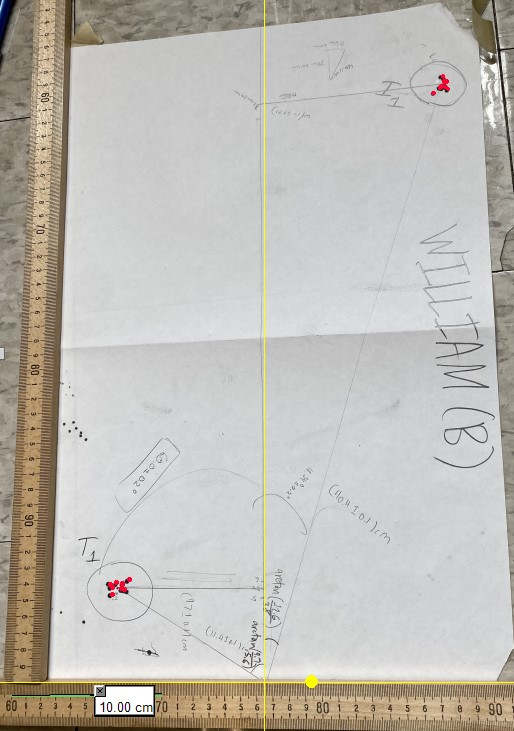
\includegraphics[width=300pt]{landingpoints.jpg}}
\captionof{figure}{Landing Points}
\end{figure}
\end{center}

Using a ruler, we measured the distances to be $\triangle{d}_{X\rightarrow{}T_{1}} = 11.4\pm0.1cm$ and $\triangle{d}_{X\rightarrow{}I_{1}} = 40.4\pm0.1cm$.

\pagebreak

\subsection{Question 2}
Determine the angle between the line XT1 and the x-axis as well as between XI1 and x-axis. Mention the method by which you determine the angles and show work if necassary.

\subsubsection{Calculating for $T_{1}$ and $I_{1}$}
Inserting the following data into Logger Pro:
\begin{center}
\begin{figure}[H]
\centering
\fbox{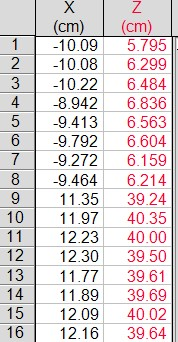
\includegraphics[width=150pt]{datapoints.jpg}}
\captionof{figure}{Image Analysis Landing Points Relative to \textbf{Point X}\\First 8 (for $T_{1}$) Next 8 (for $I_{1}$}
\end{figure}
\end{center}
Using this data and a GDC, can be made to find the average of these points. $T_{1} = (6.369\pm0.301cm, -9.659\pm0.427cm)$ and $I_{1} = (39.756\pm0.327cm, 11.958\pm0.280cm)$. We can then calculate for $\theta{}$ using the trigonometric relationship $\tan{\theta{}} = \ce{\frac{opp}{adj}}$.

\pagebreak
\subsubsection{Solving for Angles}
The percent uncertainty for:\\
$\sigma{}T_{1x} = \frac{0.301cm}{6.369cm} * 100\% = \pm4.73\%$\\
$\sigma{}T_{1y} = \frac{0.427cm}{-9.659cm} * 100\% = \pm4.42\%$\\
$\sigma{}I_{1x} = \frac{0.327cm}{39.756cm} * 100\% = \pm0.823\%$\\
$\sigma{}I_{1y} = \frac{0.280cm}{11.958cm} * 100\% = \pm2.34\%$


\begin{center}

\begin{tabular}{c l}
\hline

\raisebox{-0.5\totalheight}{\fbox{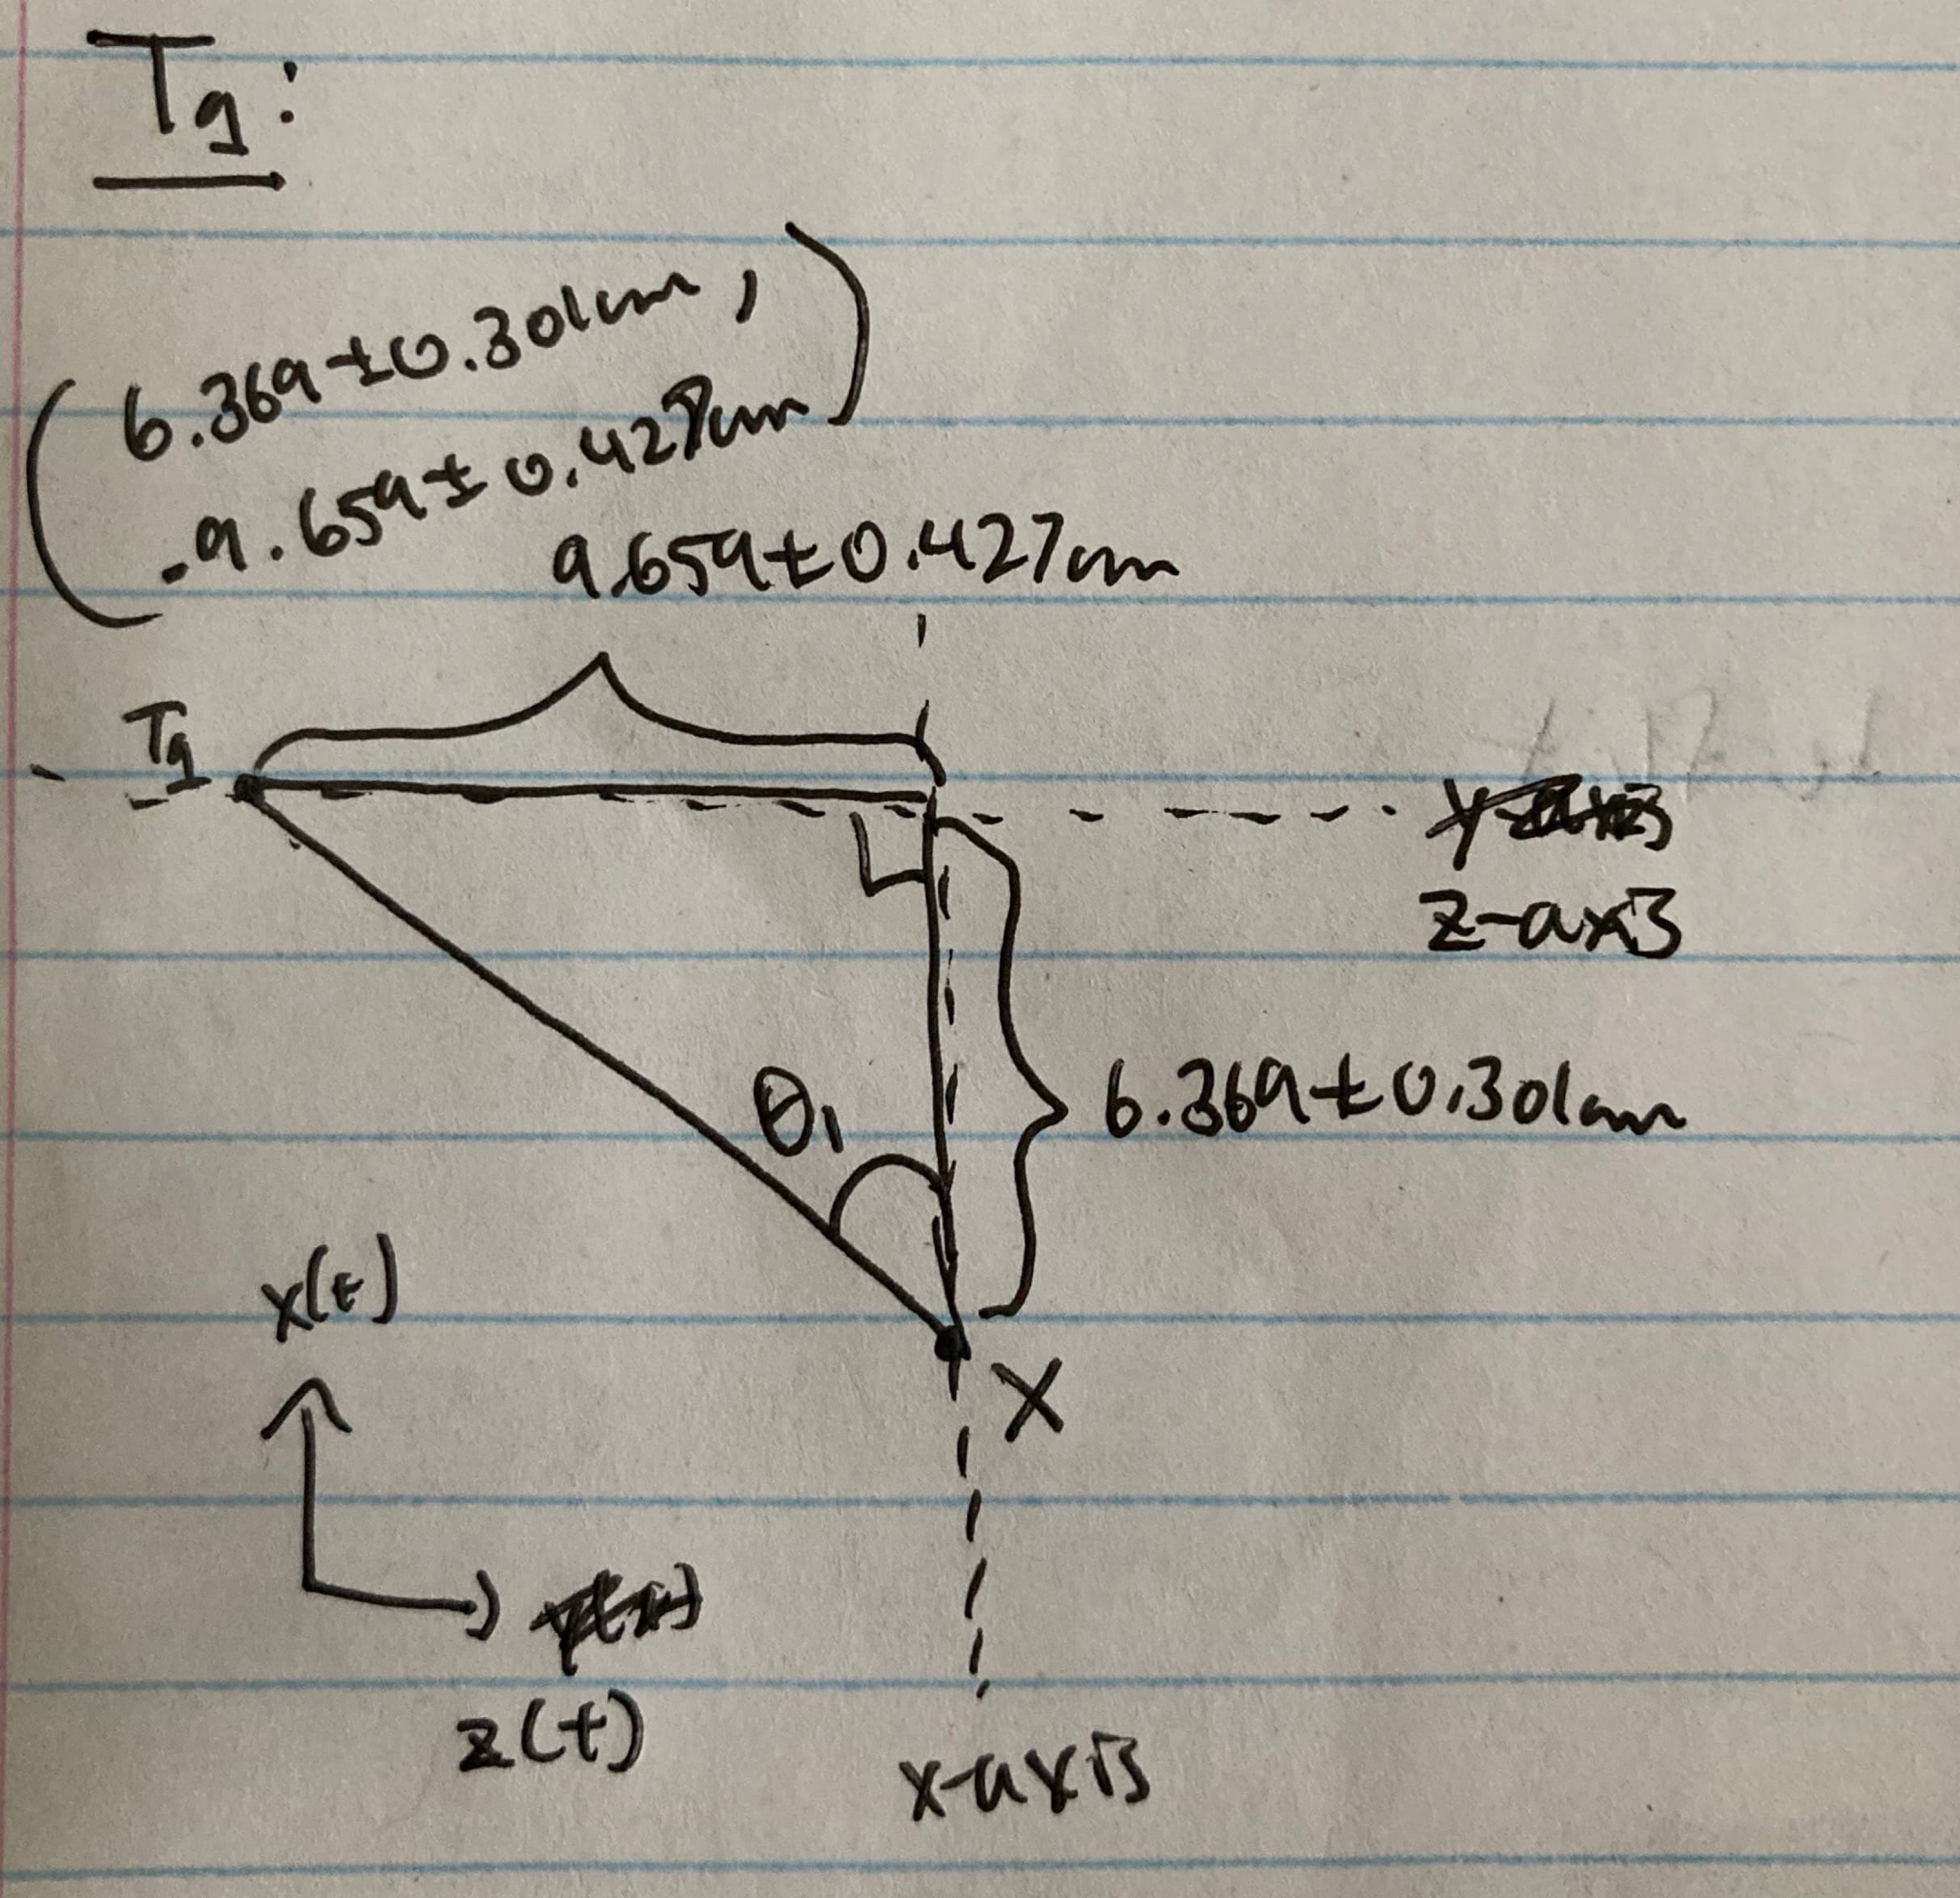
\includegraphics[width=0.4\textwidth]{T1Diagram.jpg}}} & 
{$\!\begin{aligned}
\theta{}_{T_{1}} &= \arctan{(\ce{\frac{T_{1y}}{T_{1x}}})}\\
&= \arctan{(\frac{9.659\pm0.427cm}{6.369\pm0.301cm})}\\
&= \arctan{(\frac{9.659cm\pm4.42\%}{6.369cm\pm4.73\%})}\\
&= \arctan{(1.516...\pm9.15\%)}\\
&\ce{Find uncertainty after arctan function}\\
&= 0.89785...\pm\frac{9.15\%/100\% * 0.89785...}{1 + (0.89785...)^{2}}\\
&= 0.89785...\pm0.045485...rad\\
&= 0.90\pm0.04rad
\end{aligned}$}\\
\hline
\raisebox{-0.5\totalheight}{\fbox{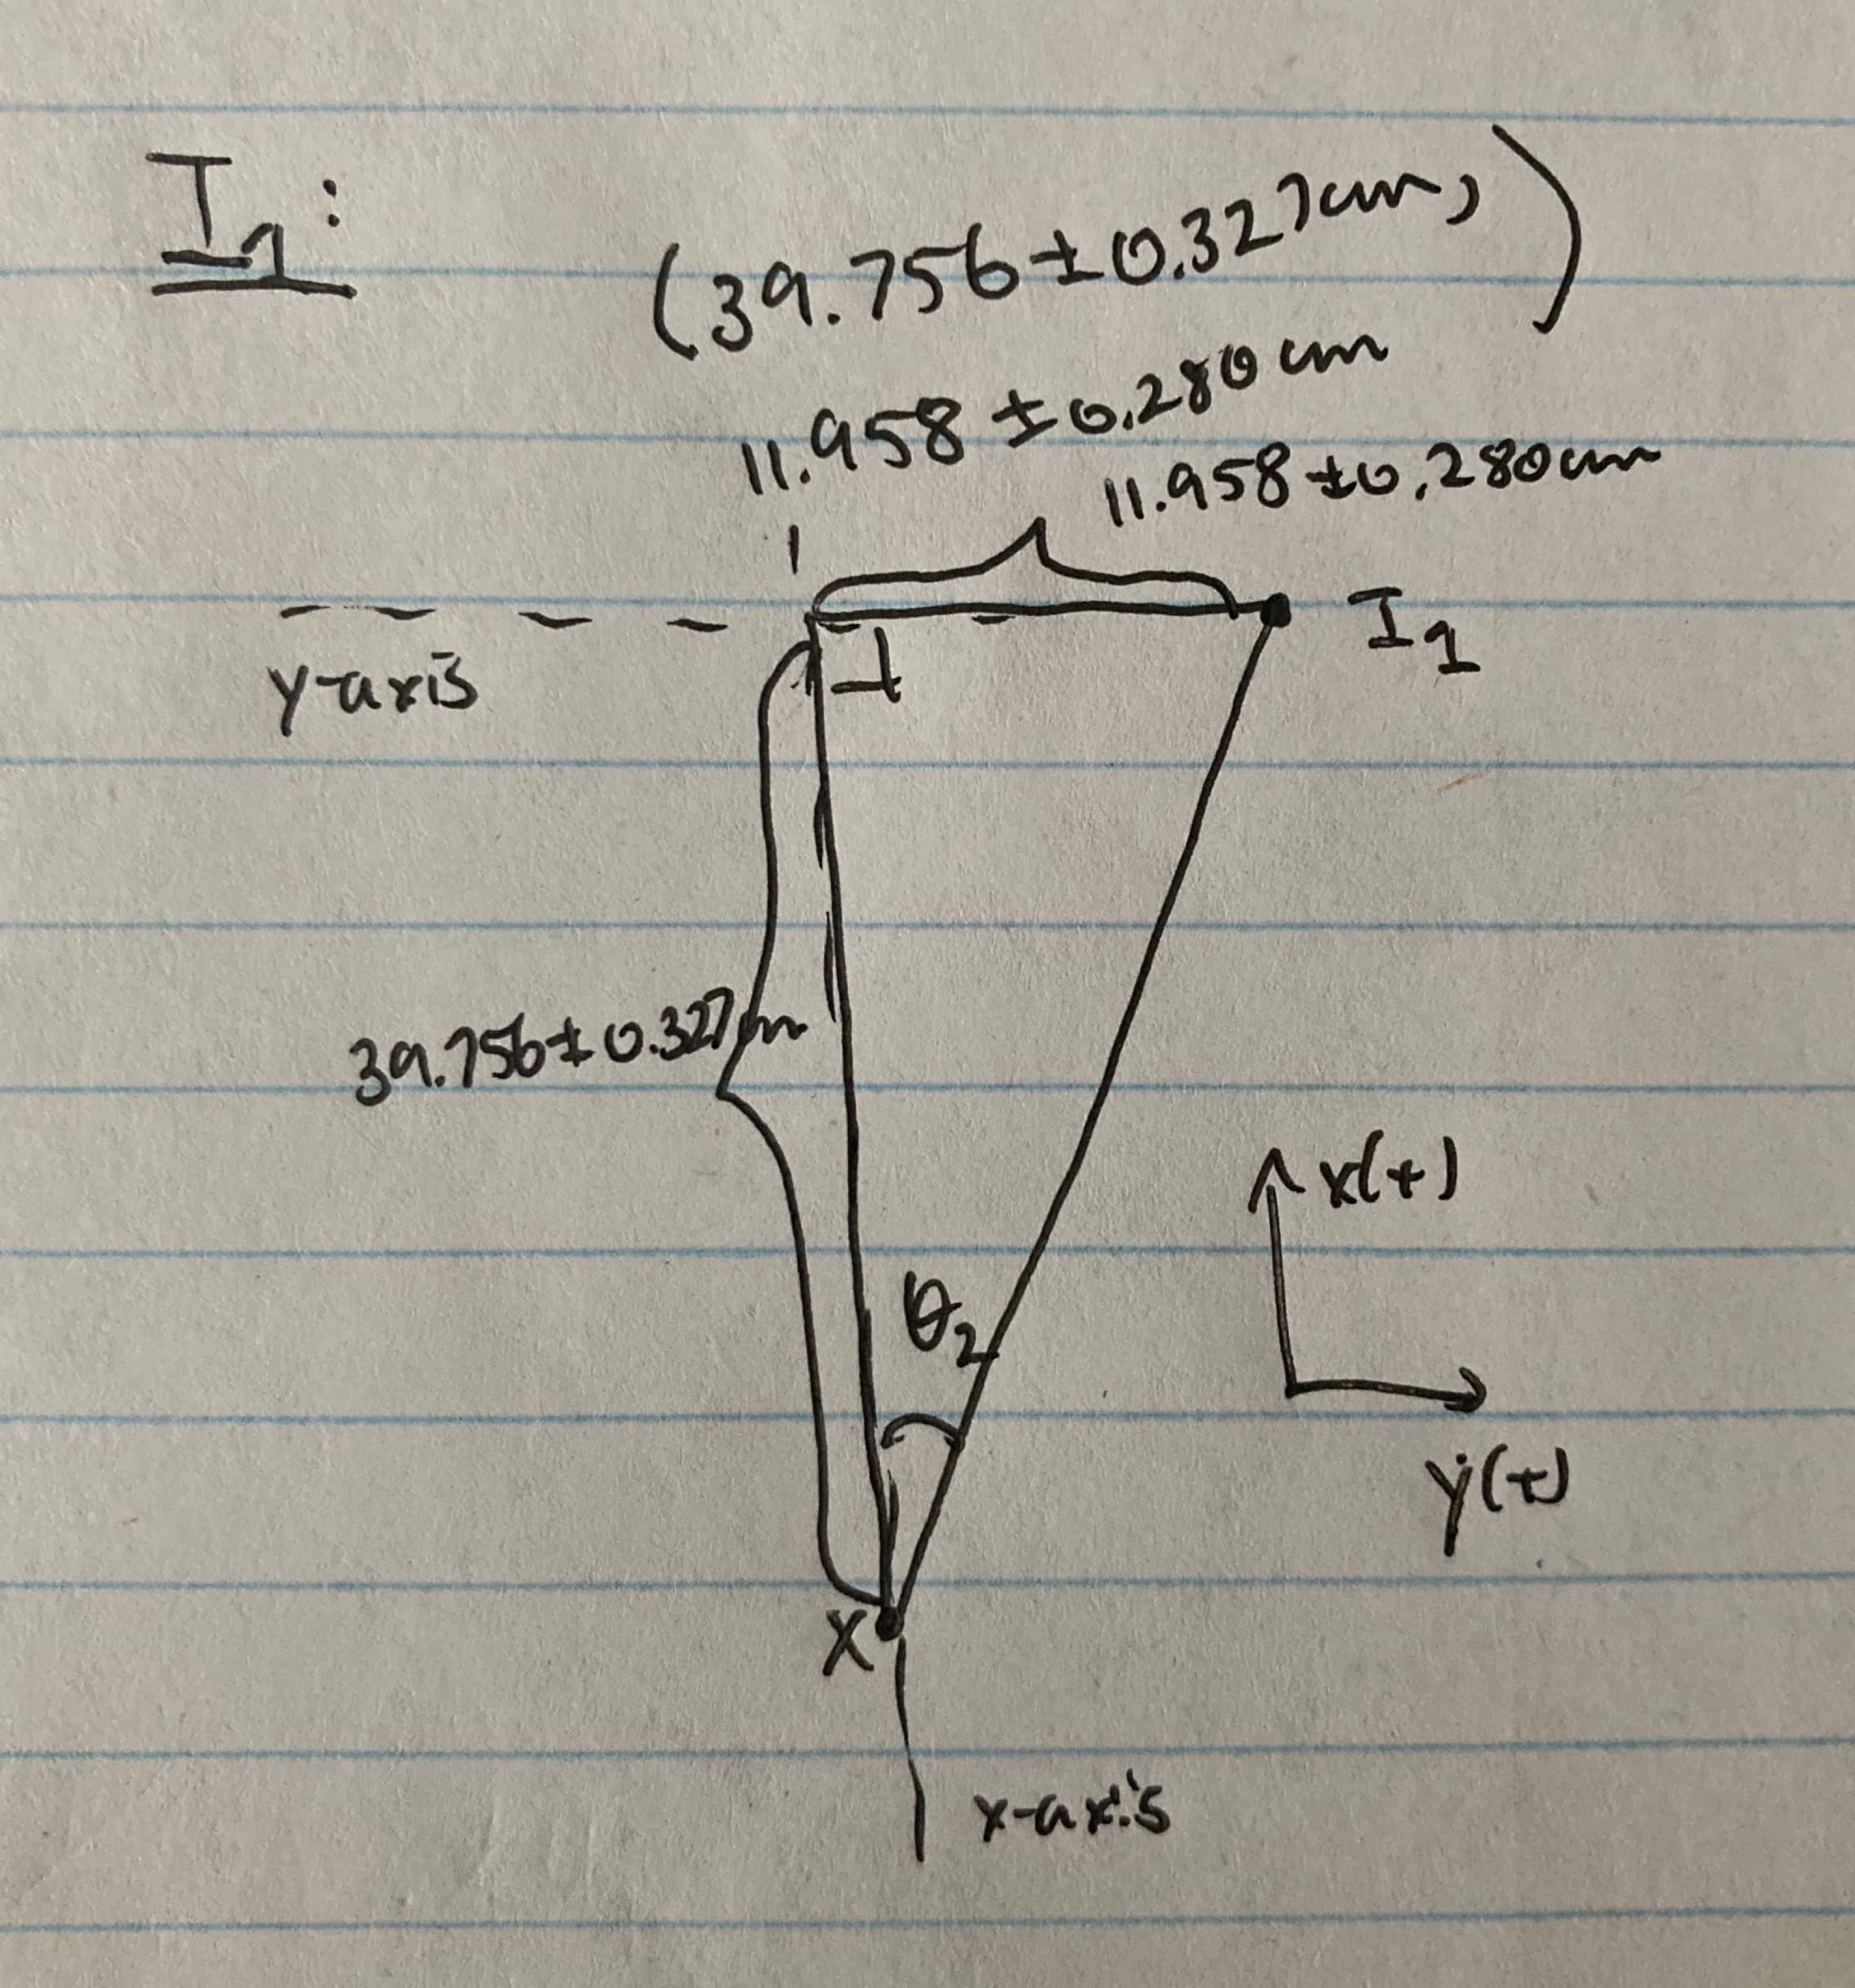
\includegraphics[width=0.4\textwidth]{I1Diagram.jpg}}} & 
{$\!\begin{aligned}
\theta{}_{I_{1}} &= \arctan{(\ce{\frac{I_{1y}}{I_{1x}}})}\\
&= \arctan{(\frac{11.958\pm0.280cm}{39.756\pm0.327cm})}\\
&= \arctan{(\frac{11.958cm\pm2.34\%}{39.756cm\pm0.823\%})}\\
&= \arctan{(0.3008...\pm3.163\%)}\\
&\ce{Find uncertainty after arctan function}\\
&= 0.2922...\pm\frac{3.163\%/100\% * 0.2922...}{1 + (0.2922...)^{2}}\\
&= 0.2922...\pm0.00851...rad\\
&= 0.292\pm0.006rad
\end{aligned}$}\\
\hline
\end{tabular}
\end{center}


Therefore the angles between the line XT1 and x-axis is $0.90\pm0.04rad$ and line XI1 and x-axis is $0.292\pm0.006rad$.

\pagebreak

\subsection{Question 3}
Using your knowledge of the principle of conservation of energy and of projectile motion, determine the initial speed of the incident ball jus tbefor ehte collision as wel as the final speed of both balls just after the collision. Show all proper equations and manipulations for full marks.













\end{document}
